% ---------------------------------------------------------------------
% --- Arquivo principal e os demais serao os dos capitulos.
% --- EXPRESSÔES ENTRE <> DEVERÃO SER COMPLETADAS COM A INFORMAÇÂO ESPECÍFICA DO TRABALHO 
% ---------------------------------------------------------------------

\documentclass[ruledheader]{abnt_UFF}

%==\usepackage[colorlinks]{hyperref}
%\usepackage[printonlyused,withpage]{acronym}

%---pacotes para hiphenizacao e acentuacao em portugues
\usepackage[utf8]{inputenc}
\usepackage[brazil]{babel}
\usepackage[T1]{fontenc}


%---fornece a capacidade de criar hiperlinks no documento
%\usepackage[dvips,colorlinks=False, pdfstartview=FitV,citecolor=green,urlcolor=black,plainpages=false, pdftitle={Dissertação de Mestrado Yona Lopes}]{hyperref}%backref,
\usepackage[hidelinks, breaklinks, colorlinks=false, pdfstartview=FitV, linkcolor=black, citecolor=green,urlcolor=black,plainpages=false]{hyperref} % usar  hidelinks para esconder os links, continuara o link mas sem aparecer cor ou borda

\usepackage[breaklinks]{hyperref} % Problema quando o nome da figura/tabela/seção eh grande
%\usepackage[dvips,pdfstartview=FitV]{hyperref}%backref,
%\usepackage[dvips]{color}
	
%---pacotes para criacao de index
\usepackage{makeidx}
%\usepackage[pdftex,colorlinks=true, pdfstartview=FitV, linkcolor=black, citecolor=black,urlcolor=black,plainpages=false]{hyperref}
\usepackage{pdfcolmk}

%--- pacote para figuras
\usepackage{epsf}
\usepackage{epsfig,graphicx}
\usepackage{subfigure}


%--- pacote de simbolos
\usepackage{latexsym}
%\usepackage{textcomp}

%--- simbolos matematicos
\usepackage{amsmath}
%\usepackage{amssymb}

%----- códigos fonte
\usepackage{listings}
% opções do pacote listings
\lstset{numbers=left, language=java, stepnumber=1, firstnumber=1, numberstyle=\tiny, extendedchars=true, breaklines=true, frame=tb, basicstyle=\footnotesize, stringstyle=\ttfamily, showstringspaces=false backgroundcolor=\color{gray}}

\newcommand\JSONnumbervaluestyle{\color{blue}}
\newcommand\JSONstringvaluestyle{\color{red}}

% switch used as state variable
\newif\ifcolonfoundonthisline

\makeatletter

\lstdefinestyle{shared}
{
	breaklines=true,
	tabsize=2,
	columns=flexible,
	morestring          = [s]{"}{"},
	stringstyle         = \ifcolonfoundonthisline\JSONstringvaluestyle\fi,
}

\lstdefinestyle{json}
{
	style=shared,
	showstringspaces    = false,
	keywords            = {false,true},
	alsoletter          = 0123456789.,
	MoreSelectCharTable =%
	\lst@DefSaveDef{`:}\colon@json{\processColon@json},
	basicstyle          = \ttfamily,
	keywordstyle        = \ttfamily\bfseries,
}

\lstdefinestyle{python}
{
	style=shared,
	language={Python},
	%alsolanguage={[Sharp]C},
	basicstyle=\small\tt,
	keywordstyle=\color{blue},
	commentstyle=\color[rgb]{0.13,0.54,0.13},
}

% flip the switch if a colon is found in Pmode
\newcommand\processColon@json{%
	\colon@json%
	\ifnum\lst@mode=\lst@Pmode%
	\global\colonfoundonthislinetrue%
	\fi
}

\lst@AddToHook{Output}{%
	\ifcolonfoundonthisline%
	\ifnum\lst@mode=\lst@Pmode%
	\def\lst@thestyle{\JSONnumbervaluestyle}%
	\fi
	\fi
	%override by keyword style if a keyword is detected!
	\lsthk@DetectKeywords% 
}

% reset the switch at the end of line
\lst@AddToHook{EOL}%
{\global\colonfoundonthislinefalse}

\makeatother

% pacote para posicionamento de tabelas e figuras
\usepackage{float}
\restylefloat{table}


%--- pacote para gerar pseudo-codigo
%\usepackage{algorithm}
%\usepackage{algorithmic}
% \usepackage[linesnumbered,boxed,lined]{algorithm2e} 
\usepackage[algoruled,portuguese,linesnumbered]{algorithm2e} 
%\floatname{algorithm}{Algoritmo}

%--- outros pacotes
\usepackage{url}
\usepackage{longtable}
\usepackage{lscape}

%\usepackage[notbib, notlof, notlot]{tocbibind}

%Tabela Colorida e pacotes de tabela
%\usepackage{colortbl}
\usepackage{array}

%--- Acronyms
%\usepackage{acronym}
\usepackage[printonlyused,withpage]{acronym}

\usepackage{multicol}
\usepackage{multirow}
\usepackage{rotating}

%--- Notes
\usepackage{todonotes}

\hyphenation{
a-de-qua-da-men-te 
di-men-sio-na-men-to 
re-di-re-cio-na
}

%---------usando tipo de fonte padrao
\renewcommand{\ABNTchapterfont}{\bfseries\fontfamily{cmr}\fontseries{b}\selectfont}
\renewcommand{\ABNTsectionfont}{\bfseries\fontfamily{cmr}}

\newcommand{\todot}[1]{\todo[color=green!40,fancyline]{#1}}


\makeindex
% --- -----------------------------------------------------------------
% --- Documento Principal.
% --- -----------------------------------------------------------------
%\usepackage[pdftex]{hyperref}
%\hypersetup{colorlinks, sitecolor=black, pdftex}
\begin{document}

% --- -----------------------------------------------------------------
% --- Titulo, abstract, dedicatorias e agradecimentos.
% --- Indice geral, lista de figuras e tabelas.
% --- -----------------------------------------------------------------

% --- -----------------------------------------------------------------
% --- Elementos usados na Capa e na Folha de Rosto.
% --- EXPRESSES ENTRE <> DEVERO SER COMPLETADAS COM A INFORMAO ESPECFICA DO TRABALHO
% --- E OS SMBOLOS <> DEVEM SER RETIRADOS 
% --- -----------------------------------------------------------------
\autor{NICOLAS DE SOUSA TEODOSIO E VICTOR HUGO NOVAIS RODRIGUES} % deve ser escrito em maiusculo

\titulo{ANÁLISE DE SENTIMENTO E MINERAÇÃO DE OPINIÕES APLICADO NO TWITTER} % deve ser escrito em maiusculo

\instituicao{INSTITUTO INFNET} % deve ser escrito em maiusculo

\orientadora{CASSIUS FIGUEIREDO}% deve ser escrito em maiusculo - preencher com o nome do seu orientador

%\coorientador{NOME} %preencher se houver.

\local{RIO DE JANEIRO} % deve ser escrito em maiusculo

\data{2016} % ano da defesa

\comentario{Trabalho de Conclusão de Curso apresentado ao Programa de Graduação em Engenharia da Computação do \mbox{Instituto Infnet} como parte dos requisitos necessários à obtenção do título de \mbox{Bacharel em Engenharia da Computação}.}%preencha com a sua area de concentracao


% --- -----------------------------------------------------------------
% --- Capa. (Capa externa, aquela com as letrinhas douradas)(Obrigatorio)
% --- ----------------------------------------------------------------
\capa

% --- -----------------------------------------------------------------
% --- Folha de rosto. (Obrigatorio)
% --- ----------------------------------------------------------------
\folhaderosto


\pagestyle{ruledheader}
\setcounter{page}{1}
\pagenumbering{roman}

% --- -----------------------------------------------------------------
% --- Ficha Catalográfica. (Obrigatorio)
% --- ----------------------------------------------------------------
%
%\cleardoublepage
%\thispagestyle{empty}
%\vspace*{130mm}
%
%\begin{flushright}
%
%\hspace{8em}
%\fbox{\begin{minipage}{10cm}

%....

%\end{minipage}}
%
%\end{flushright}
%\newpage

% --- -----------------------------------------------------------------
% --- Termo de aprovacao. (Obrigatorio)
% --- ----------------------------------------------------------------


\cleardoublepage
\thispagestyle{empty}

\vspace{-60mm}

\begin{center}
   {\large NICOLAS DE SOUSA TEODOSIO E VICTOR HUGO NOVAIS RODRIGUES}\\
   \vspace{7mm}

  ANÁLISE DE SENTIMENTO E MINERAÇÃO DE DADOS APLICADO NO TWITTER\\
%   \vspace{10mm}
 \vspace{8mm}  %diminui para ajustar a data que estava pulando para outra folha
\end{center}

\noindent
\begin{flushright}
\begin{minipage}[t]{8cm} 
%\begin{minipage}{\columnwidth}

Trabalho de Conclusão de Curso apresentado ao Programa de Graduação em Engenharia da Computação do \mbox{Instituto Infnet} como parte dos requisitos
necessários à obtenção do título de \mbox{Bacharel em Engenharia da Computação}

\end{minipage}
\end{flushright}
\vspace{ 5mm}  %original 1cm
\noindent
Aprovada em XX agosto de 2016. \\
\begin{flushright}
  \parbox{15cm}
  {
  \begin{center}
  BANCA EXAMINADORA \\
  \vspace{5mm}
  \rule{11cm}{.1mm} \\
	Profº. Cassius Figueired, M.Sc. - Orientadora \\ 
	Instituto INFNET \\
  \vspace{5mm}
  \rule{11cm}{.1mm} \\
    Profª. XXXX, titulacao.  \\
    Universidade \\
  \vspace{5mm}
  \rule{11cm}{.1mm} \\
    Profº. xxx, TITULACAO \\
    Universidade\\
  \end{center}
  }
\end{flushright}
\begin{center}
  \vspace{4mm} % 
 Rio de Janeiro \\
  %\vspace{6mm}
  2016
\end{center}

% --- -----------------------------------------------------------------
% --- Dedicatoria.(Opcional)
% --- -----------------------------------------------------------------
\cleardoublepage
\thispagestyle{empty}
\vspace*{200mm}

\begin{flushright}
{\em 
À minha família.
%Dedicatória(s): À blá blá%Elemento opcional onde o autor presta homenagem ou dedica seu trabalho (ABNT, 2005).
}
\end{flushright}
\newpage


% --- -----------------------------------------------------------------
% --- Agradecimentos.(Opcional)
% --- -----------------------------------------------------------------
\pretextualchapter{Agradecimentos}
\hspace{5mm}
Agradeço, inicialmente, 

% --- -----------------------------------------------------------------
% --- Resumo em portugues.(Obrigatorio)
% --- -----------------------------------------------------------------
\begin{resumo}

Atualmente a internet e micro blogs em geral têm se tornado uma ferramenta de comunicação poderosa entre usuários de Internet. Bilhões de pessoas compartilham informações e opiniões todos os dias, fazendo desse espaço um ótimo campo de pesquisas comercias, acadêmicas e sociológicas.  Como o fenômeno é relativamente recente – o Twitter foi criado apenas em 2006 – ainda existem poucas pesquisas destinadas ao tema., especialmente quando o idioma de estudo é o português. O objetivo deste trabalho é explorar a análise de sentimento aplicada à mineração de opiniões em \emph{tweets} de língua portuguesa.

{\hspace{-8mm} \bf{Palavras-chave}}: Análise de sentimento, mídias sociais, twitter,mineração de dados , mineração de opiniões, processamento de linguagem natural, naive bayes.

%redefine todas siglas para não usado
\acresetall

\end{resumo}

% --- -----------------------------------------------------------------
% --- Resumo em lingua estrangeira.(Obrigatorio)
% --- -----------------------------------------------------------------
\begin{abstract}


{\hspace{-8mm} \bf{Palavras-chave}}: xxxxxxx.


%redefine todas siglas para não usado
\acresetall

\end{abstract}

% --- -----------------------------------------------------------------
% --- Lista de figuras.(Opcional)
% --- -----------------------------------------------------------------
\cleardoublepage
\listoffigures
\label{listadefiguras}
\acresetall

% --- -----------------------------------------------------------------
% --- Lista de tabelas.(Opcional)
% --- -----------------------------------------------------------------
\cleardoublepage
\label{listadetabelas}
\listoftables
\cleardoublepage
\acresetall

% --- -----------------------------------------------------------------
% --- Lista de abreviatura.(Opcional)
%Elemento opcional, que consiste na relação alfabética das abreviaturas e siglas utilizadas no texto, seguidas das %palavras ou expressões correspondentes grafadas por extenso. Recomenda-se a elaboração de lista própria para cada %tipo (ABNT, 2005).
% --- ----------------------------------------------------------------
\cleardoublepage
\pretextualchapter{Lista de Abreviaturas e Siglas} %%%Baixo Exemplo. Apagar e colocar os proprios em ordem alfabetica
\begin{acronym}[MCAA]

 \acro{IED}{\textit{Intelligent Electronic Device}}
 \acro{TC} {Transformador de Corrente}
 \acro{TP} {Transformador de Potencial}
 \acro{TPAA} {\textit{Two Party Application Association}}
\end{acronym}

% --- -----------------------------------------------------------------
% --- Sumario.(Obrigatorio)
% --- -----------------------------------------------------------------
\pagestyle{ruledheader}
\tableofcontents
\acresetall



% --- -----------------------------------------------------------------
% --- Insercao dos capitulos.
% --- -----------------------------------------------------------------
\pagestyle{ruledheader}
\setcounter{page}{1}
\pagenumbering{arabic}

\inputencoding{utf8}

\chapter{Introdução} \label{cap:1}

Através do fenômeno da popularização da Internet vivemos hoje um período conhecid como "Era da conhecimento" \cite{lastres1999informaccao}. A diminuição das distâncias entre bilhões de pessoas por todo o mundo criou um verdadeiro \textit{boom} em nossas vidas. A sociedade em que vivemos possui hoje uma facilidade ao acesso da informação nunca antes visto. 
Nesse contexto, redes sociais conhecidas, como Facebook e Twitter se tornaram bastante populares por permitirem a seus usuários acesso à um ambiente onde todos possuem voz e vez para se expressar e por consequência, para se informar sobre tudo que acontece no mundo.
Através de \ac{API} disponibilizadas por essas redes sociais, possuímos fácil acesso à um grande volume de opiniões catalogadas - através de \textit{hashtags} - que podem ser utilizadas em pesquisas de opinião sobre um tema ou assunto específico. Tal cenário apresenta-se como uma grande oportunidade de pesquisa em áreas acadêmicas, sociais e comerciais.
Porém, quando o objeto de estudo é a língua portuguesa, nota-se que a mesma carece de trabalhos e implementações na área de mineração de opiniões e análise de sentimento. Alguns motivos explicam essa carência: poucos investimentos na área de ciência e engenharia da computação em nosso país e a grande dificuldade que a língua portuguesa apresenta ao ser interpretada através de processamento de linguagem natural. \cite{santos2000projecto}


\section{Motivação e Objetivos}\label{sec:1_inicio}
%A motivação deste trabalho é explorar o potencial contido no conteúdo digital gerado todos os dias em redes sociais por %usuários brasileiros. Tais dados possuem informações valiosas que podem ser explorados de inúmeras maneiras



\section{Principais contribuições}\label{sec:1_principais_contribuicoes}

\section{Recursos utilizados}\label{sec:1_recursos_utilizados}

\section{Organização do trabalho}\label{sec:1_org}

Este trabalho está estruturado em 5 capítulos da seguinte forma: no Capítulo~\ref{cap:1}, para embasamento teórico, são apresentados os conceitos de ... Neste capítulo, os conceitos relacionados a ..., dentre outros, são descritos. Em seguida, no Capítulo XX , é feita uma análise sobre os principais trabalhos relacionados ao uso dos ... . No Capítulo~\ref{cap:2}, os conceitos do arcabouço utilizado ... , são descritos. Nesse capítulo são mostrados os motivos para a escolha desse arcabouço, .... A proposta XXX é apresentada no Capitulo~\ref{cap:3}, onde a arquitetura da proposta é detalhada, assim como seus componentes e algoritmos. Em seguida, o Capítulo~\ref{cap:4} apresenta as ferramentas utilizadas para implementação da proposta, o ambiente implementação, a descrição dos experimentos e os principais resultados obtidos com o XXX, assim como a análise dos valores encontrados. Por fim, o Capítulo~\ref{cap:5} conclui este trabalho, ressaltando os objetivos alcançados com as propostas. As principais vantagens e desvantagens da proposta são discutidas, assim como alguns trabalhos futuros que podem ser desenvolvidos. 

\chapter{Referencial Teórico}\label{cap:referencial_teorico}

\section{Twitter}\label{sec:twitter}

* Como começou
* Objetivo (visão) do Twitter
* Princípios 140 caracteres, hashtags
* Quantidade de usuários ativos, alcance, volume de informações
* Relevância para estudos estatísticos de natureza comportamental

O Twitter é conhecido como um \textit{microblog} fundado em março de 2006 por Jack Dorsey, Evan Williams e Biz Stone. Ele consiste em pequenas publicações de até 140 caracteres, conhecidas como \textit{tweet}, que tem como objetivo possibilitar que o usuário se expresse de forma rápida e resumida. No corpo de um \textit{tweet}, o usuário pode fazer uso de marcadores conhecidos como \textit{hashtags}\cite{waite2012paperback}, para vincular aquela mensagem à um tópico específico.
%\cite{arneromannkurrik2013} A referência tava no texto, mas não to no .bib


\section{Mineração de opinião}\label{sec:mineracao_dados}

* O que é?
* Exemplos no mercado
* Etapas(http://www.inf.ufsc.br/~alvares/INE5644/MineracaoOpiniao.pdf)

\section{API}\label{sec:api}
* O que é
* APIs mais utilizadas no mundo (case do twitter)
* Papel de uma API para integração de serviços (achar referência foda)

\section{Processamento de linguagem natural}\label{sec:nlp}
* Linguagem natural (foto da matéria de autômato do Aquino?)
* Processamento de linguagem natural
* Dificuldades dentro da nossa área de estudo

\section{Análise de sentimento}\label{sec:analise_sentimento}
* Definição
* Objetivo
* Premissas
* Exemplos e cases de sucesso


\section{Naive Bayes}\label{sec:naive_bayes}
* O que é o Naive Bayes
* Demonstração matemática do algoritmo
* Uso dele em analise de sentimento/classificação


\\ \emph{Naive Bayes} é um algoritmo probabilístico. Baseado no teorema de bayes. $$ P(A \mid B) = \frac{P(B \mid A) \, P(A)}{P(B)} $$ onde se infere qual é a probabilidade de um evento A dado um evento B. Porém nesse trabalho é utilizado o \emph{Naive Bayes} e sua diferença para o teorema de Bayes é assumir que a posição das palavras que aparecem no texto não importa, daí é acrescentado o \emph{naive}(ingênuo) ao teorema.
\\ Como visto em \cite{lucca2013implementaccao} o algoritmo computa qual a probabilidade de uma frase, denominada de documento pertencer a uma determinada classe(polaridade) \emph{P(c/d)}, a partir da probabilidade a \emph{priori} de \emph{P(c)} do documento pertencer a esta classe e da probabilidades condicionais de cada termo \emph{tk} ocorrer em um documento da mesma classe. O algoritmo tem como objetivo encontrar a melhor classe para um documento maximizando a probabilidade a\emph{posteriori} conforme a equação abaixo, onde $ n_{d} $ é o número de termos no documento \emph{d}. $$ C_{map}= argmax_{c \epsilon C}P(c|d)=argmax_{c \epsilon C}P(c)\prod 1sksn_{d}P(t_{k}/d) $$
\chapter{Proposta} \label{cap:proposta}

Como visto no Capítulo 2, existe uma corrente dentro da Mineração de Opinião que vem desenvolvendo maneiras de explorar o conteúdo digital gerado pela nossa sociedade todos os dias em redes sociais, através de técnicas utilizando Processamento de Linguagem Natural e \textit{Machine Learning}, principalmente. Com este fato surge a oportunidade de explorar novas ferramentas na
solução de problemas que envolvem pesquisas de opinião de forma geral.
Neste trabalho propõem-se um \textit{framework} que torna possível fazer pesquisas de opiniões em língua portuguesa sobre qualquer tema que seja rastreável a partir de uma \textit{hashtag} no Twitter.
Para tal é necessário que o framework criado seja capaz de:

% TODO: Colocar Lista ordenada
\begin{itemize}
	\item Coletar \textit{tweets} escritos em língua portuguesa que contenham uma determinada {hashtag} escolhida como objeto de estudo em tempo real;
	\item Armazenar as mensagens em uma base de dados;
	\item Classificar as mensagens em: negativo, neutro e positivo;
	\item Extrair \textit{insights} que auxiliem em tomadas de decisão a partir da massa de dados classificada;
\end{itemize}

Para alcançar este objetivo a proposta deste trabalho envolve passos preparatórios que permitem o pleno funcionamento do \textit{framework}.

\begin{itemize}
	\item Definir as técnicas de normalização que serão aplicadas ao texto antes da classificação;
	\item Construir base de palavras e termos classificados utilizadas como insumo para o modelo matemático;
	\item Preparar uma massa de treino para validar o modelo matemático antes da execução;
\end{itemize}

\section{Construção da base de palavras e termos}
A construção da base de dados foi feita com o intuito de melhor expressar um sentimento de uma palavra ou texto, para a utilização do algoritmo. Para isso a base foi dividida em dois arquivos, positivos e negativos. Além dessa divisão foi utilizada outas bases criadas como: Re-li(referencia), SentiLex-PT \cite{marioj.silvapaulacarvalholuissarmento2012}, base da puc \cite{freitas2013construccao}, emoticons \cite{alexanderhogenboomdaniellabalflaviusfrasincarmalissabalfranciskadejonguzaykaymak}. Todas usando a língua portuguesa ou um linguajar universal, no caso dos emoticons e já estarem polarizadas. Essas bases têm em comum é serem feitas apenas de palavras, então ficou-se a dúvida de como a classificação funcionaria posteriormente quando aplicadas a um texto que as palavras podem não estar no mesmo contexto. Ex: "O flamengo jogou muito mal, mas fico feliz pela vitória", onde tem a palavra mal que já dá um tom negativo a frase , porém ao terminar de ler a frase encontrasse as palavras feliz e vitória que tem um contexto positivo.
Com essas bases já citadas foi compreendida a necessidade de uma base mais específica para o linguajar utilizado na internet, constituído de  
gírias, abreviação e até erros de português, para isso foi criada uma base utilizando dados pegos do twitter a partir da marcação hashtagoscar2016.


\section{Coleta de dados}


\section{Armazenamento}


\section{Classificação}


\subsection{Massa de treino}


\subsection{Massa de teste}

\subsection{Algoritmo}



\subsection{Massa de treino}


\subsection{Massa de teste}


\subsection{Plataforma de análise}

\chapter{Resultados e análises}\label{cap:resultados}

Neste capítulo serão apresentados resultados obtidos e os processos necessários para a obtenção dos mesmos. Como visto anteriormente no Capitulo 2,  uma das etapas
necessárias para a Análise de Sentimento é a classificação de polaridade dos \textit{tweets}. Durante a classificação, que gera o resultado da execução do Naive Bayes, foram utilizadas diversas formas de execução que serão apresentadas durante este capítulo.

\section{Cenários e parâmetros de teste}\label{sec:cenarios}
Durante a execução dos testes para a análise de resultados o ambiente utilizado foi:
\begin{itemize}
	\item Sistema operacional: Linux Ubuntu 15.04
	\item Processador: Core i7
	\item Memória: 8GB
	\item Quantidade de \textit{tweets}: 141.798
\end{itemize}


\section{Desenvolvimento do modelo de análise}\label{sec:desenv-moda}
O primeiro teste realizado para a classificação da base obteve o seguinte resultado:
\todo{Trazer tabela  1 pra ca}
\begin{table}[]
	\caption{1º teste}
	\label{teste-1}
	\resizebox{\textwidth}{!}{%
		\begin{tabular}{|l|l|r}
			\hline
			\multicolumn{3}{|c|}{1º Teste} \\ \hline
			\multicolumn{2}{|l|}{Bases usadas} & \multicolumn{1}{r|}{Tecnicas usadas} \\ \hline
			\multicolumn{2}{|c|}{Sentilex} & \multicolumn{1}{c|}{Stopwords} \\
			\multicolumn{2}{|c|}{PUC} & \multicolumn{1}{c|}{Stemming} \\ \cline{3-3} 
			\multicolumn{2}{|c|}{ReLi} &  \\ \hline
			\multicolumn{3}{|c|}{Resultado} \\ \hline
			\multicolumn{2}{|l|}{Positivo} & \multicolumn{1}{r|}{17350} \\ \hline
			\multicolumn{2}{|l|}{Negativo} & \multicolumn{1}{r|}{15517} \\ \hline
			\multicolumn{2}{|l|}{Neutro} & \multicolumn{1}{r|}{108931} \\ \hline
			\multicolumn{2}{|l|}{Tempo} & \multicolumn{1}{r|}{311.673 segundos} \\ \hline
		\end{tabular}%
	}
\end{table}

Analisando a tabela \ref{teste-1} é visto quais as bases utilizadas, nesse caso, Reli , PUC e Sentilex, as técnicas utilizadas nesse teste, \textit{Stopwords} e \textit{Stemming}, e o resultado que de 141.798 \textit{tweets}, 17.350 foram positivos, 15.517 negativos e 108.931 neutros, levando 311,673 segundos para executar o teste.
\todo{Adicionar imagem grafico 1}
\begin{figure}[!h]
	\centering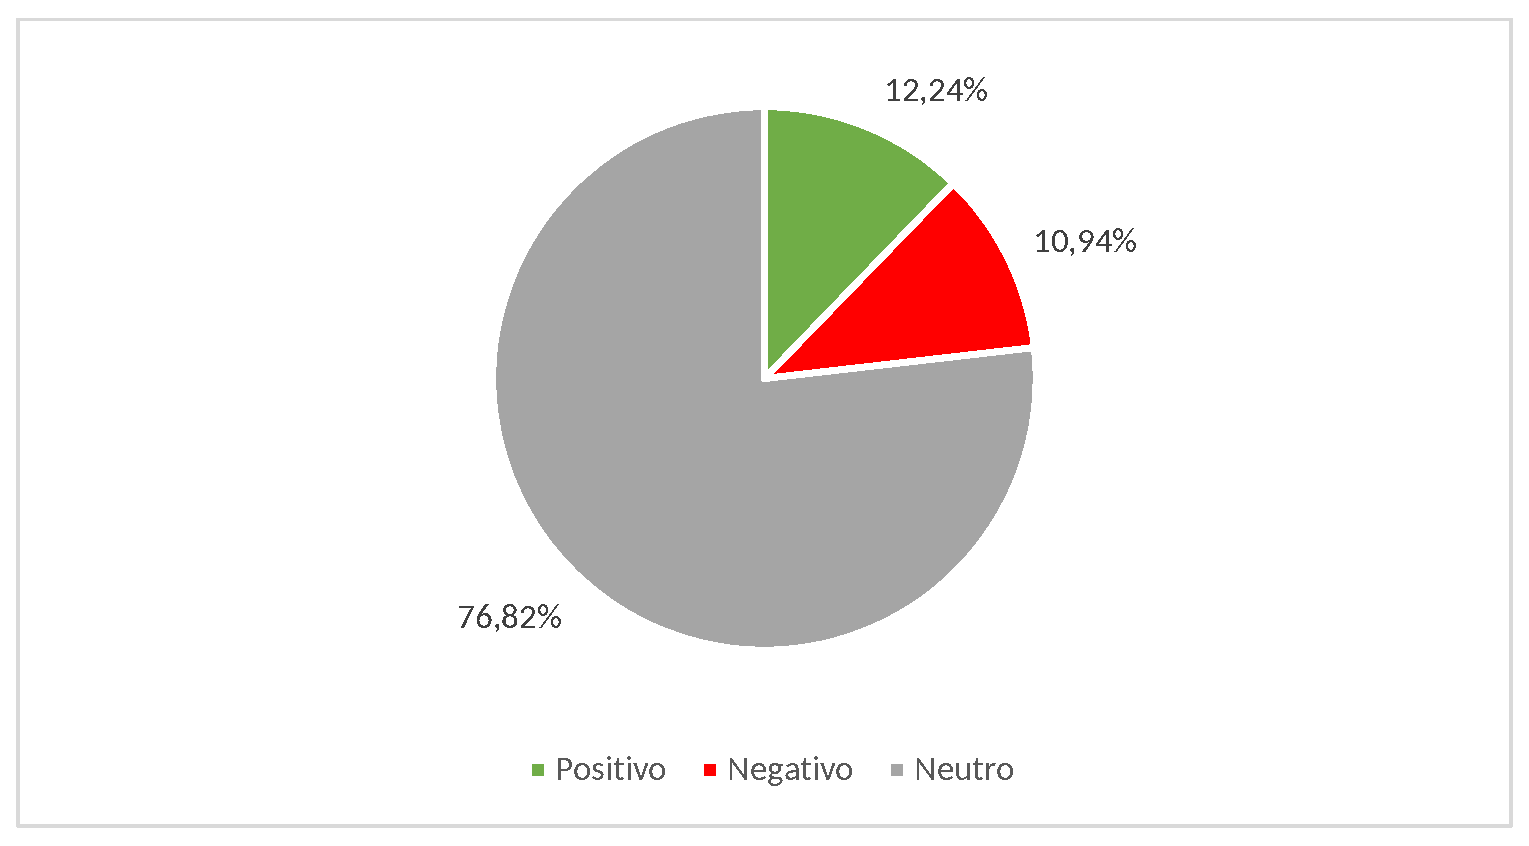
\epsfig{file=figuras/teste-1.eps, width=20cm}
	\caption{Quantidade de tweets separados por polaridade do teste 1. Fonte: Própria}
	\label{teste-graf-1}
\end{figure}

Nota-se que a quantidade de \textit{tweets} neutros é muito alta, evidenciando que o modelo ainda tem dificuldade de definir a polaridade do texto. Com base nos resultados apresentados foram realizadas as seguintes mudanças visando diminuir a ocorrência de "neutros".
 
\todo{Tabela 2 aqui}

\begin{table}[]
	\caption{2º teste}
	\label{teste-2}
	\resizebox{\textwidth}{!}{%
		\begin{tabular}{|l|l|r}
			\hline
			\multicolumn{3}{|c|}{2º Teste} \\ \hline
			\multicolumn{2}{|l|}{Bases usadas} & \multicolumn{1}{r|}{Tecnicas usadas} \\ \hline
			\multicolumn{2}{|c|}{Sentilex-Stem} & \multicolumn{1}{c|}{Stopwords-Stem} \\
			\multicolumn{2}{|c|}{PUC-Stem} & \multicolumn{1}{c|}{Stemming} \\ \cline{3-3} 
			\multicolumn{2}{|c|}{ReLi} &  \\ \hline
			\multicolumn{3}{|c|}{Resultado} \\ \hline
			\multicolumn{2}{|l|}{Positivo} & \multicolumn{1}{r|}{49263} \\ \hline
			\multicolumn{2}{|l|}{Negativo} & \multicolumn{1}{r|}{35079} \\ \hline
			\multicolumn{2}{|l|}{Neutro} & \multicolumn{1}{r|}{57456} \\ \hline
			\multicolumn{2}{|l|}{Tempo} & \multicolumn{1}{r|}{397.48 segundos} \\ \hline
		\end{tabular}%
	}
\end{table}

No 2º teste visto na tabela \ref{teste-2} é visto que a quantidade de neutro diminuiu consideravelmente, apenas aplicando a técnica de \textit{stemming} nas bases de palavras
\todo{grafico 2}
\begin{figure}[!h]
	\centering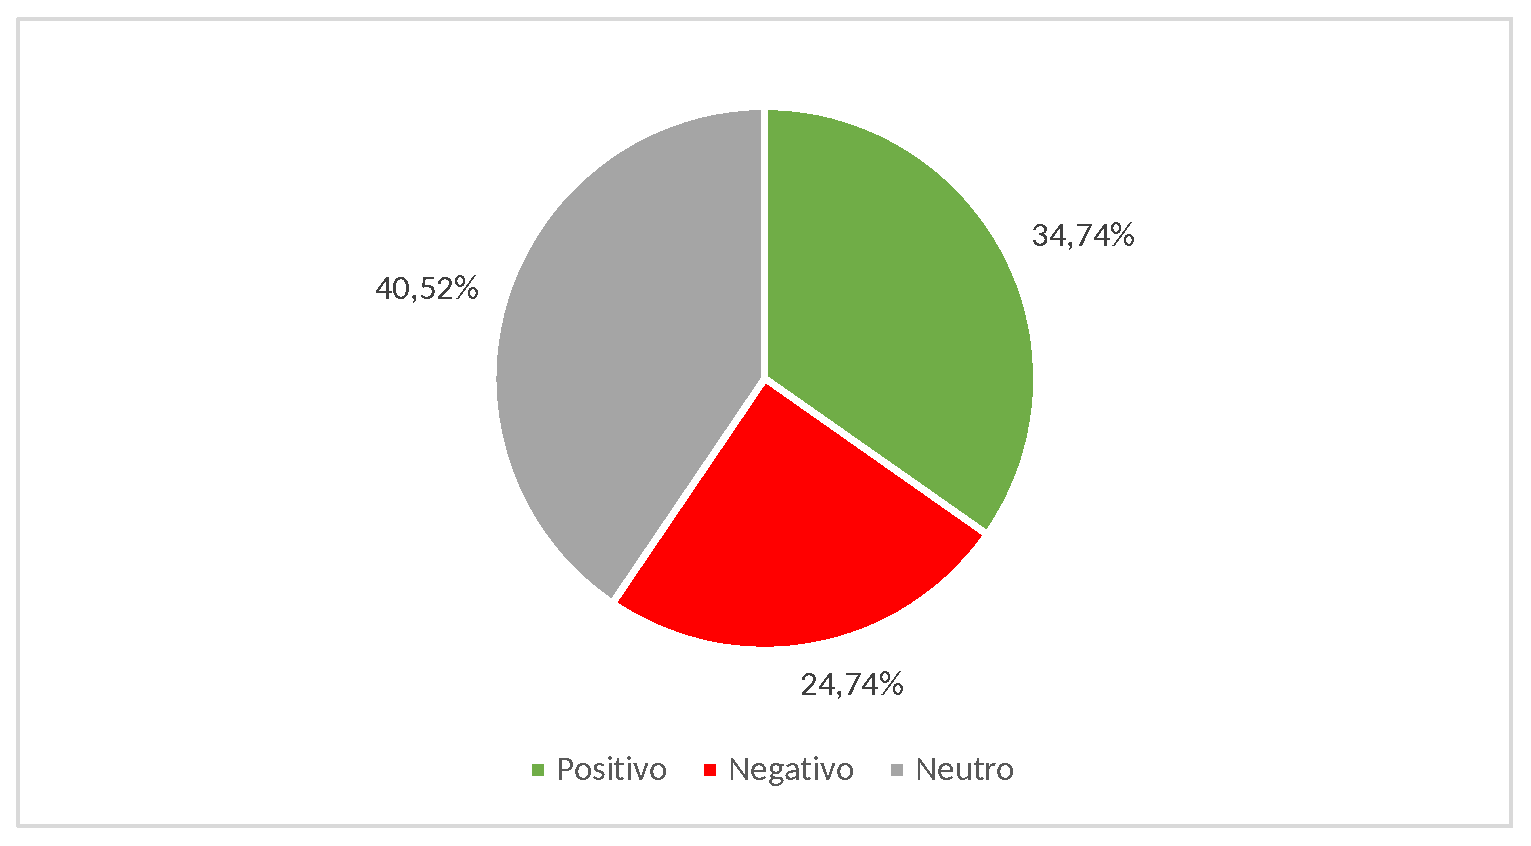
\epsfig{file=figuras/teste-2.eps, width=20cm}
	\caption{Quantidade de tweets separados por polaridade do teste 2. Fonte: Própria}
	\label{teste-graf-2}
\end{figure}

Ainda buscando a diminuição de neutros foi criada uma base de palavras mas próxima do domínio que esse trabalho propõe que é o Oscar2016, essa base contem palavras relevantes a esse evento, gerando o seguinte resultado.
\todo{colocar tabela 3 aqui}

\begin{table}[]
	\caption{3º teste}
	\label{teste-3}
	\resizebox{\textwidth}{!}{%
		\begin{tabular}{|l|l|r|}
			\hline
			\multicolumn{3}{|c|}{3º Teste} \\ \hline
			\multicolumn{2}{|l|}{Bases usadas} & Técnicas usadas \\ \hline
			\multicolumn{2}{|c|}{Oscar2016} & \multicolumn{1}{c|}{\textit{Stopwords}} \\ \hline
			\multicolumn{3}{|c|}{Resultado} \\ \hline
			\multicolumn{2}{|l|}{Positivo} & 47450 \\ \hline
			\multicolumn{2}{|l|}{Negativo} & 7210 \\ \hline
			\multicolumn{2}{|l|}{Neutro} & 87138 \\ \hline
			\multicolumn{2}{|l|}{Tempo} & 709,126 segundos \\ \hline
		\end{tabular}%
	}
\end{table}

Analisando a tabela \ref{teste-3} é visto que apenas uma base mais especializada no domínio não consegue diminuir a quantidade de neutros e ainda aumenta o tempo para a execução dos testes.
\todo{grafico 3}
\begin{figure}[!h]
	\centering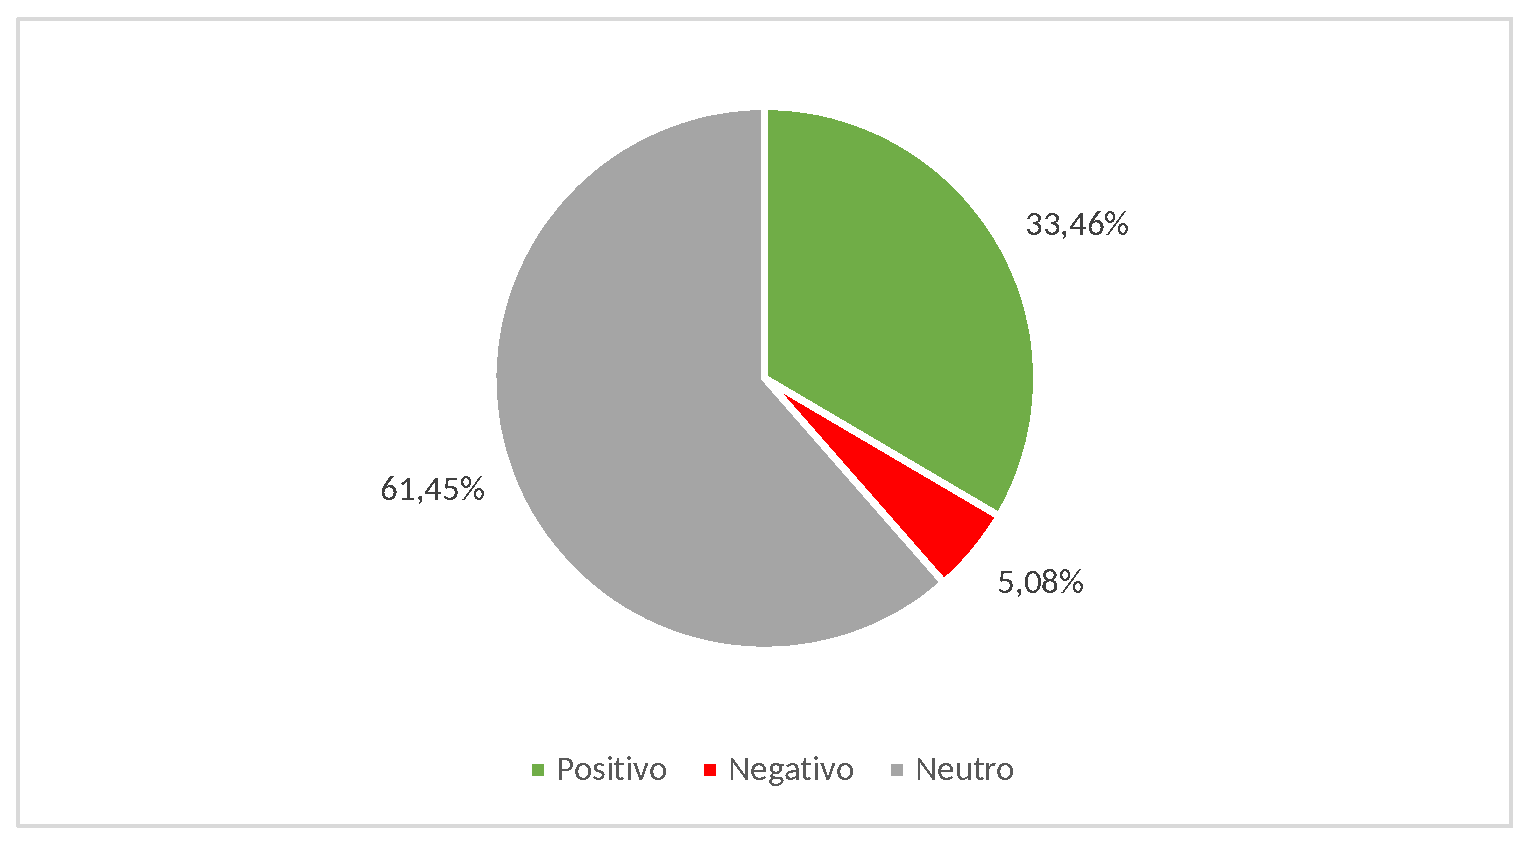
\epsfig{file=figuras/teste-3.eps, width=20cm}
	\caption{Quantidade de tweets separados por polaridade do teste 3. Fonte: Própria}
	\label{teste-graf-3}
\end{figure}

No 4º teste foi adicionada o base criada, Oscar2016, com as bases genéricas, gerando o seguinte resultado:
\begin{table}[]
	\caption{4º teste}
	\label{teste-4}
	\resizebox{\textwidth}{!}{%
		\begin{tabular}{|c|l|r}
			\hline
			\multicolumn{3}{|c|}{4º Teste} \\ \hline
			\multicolumn{2}{|l|}{Bases usadas} & \multicolumn{1}{r|}{Técnicas usadas} \\ \hline
			\multicolumn{2}{|c|}{Oscar2016} & \multicolumn{1}{c|}{Stopwords} \\
			\multicolumn{2}{|c|}{SentiLex} & \multicolumn{1}{c|}{Stemming} \\ \cline{3-3} 
			\multicolumn{2}{|c|}{PUC} & \multicolumn{1}{c}{} \\
			\multicolumn{2}{|c|}{ReLi} & \multicolumn{1}{c}{} \\ \hline
			\multicolumn{3}{|c|}{Resultado} \\ \hline
			\multicolumn{2}{|l|}{Positivo} & \multicolumn{1}{r|}{69070} \\ \hline
			\multicolumn{2}{|l|}{Negativo} & \multicolumn{1}{r|}{33461} \\ \hline
			\multicolumn{2}{|l|}{Neutro} & \multicolumn{1}{r|}{39267} \\ \hline
			\multicolumn{2}{|l|}{Tempo} & \multicolumn{1}{r|}{650.97 segundos} \\ \hline
		\end{tabular}%
	}
\end{table}

Analisando a tabela \ref{teste-4} é visto que nesse teste foi obtido a maior diminuição de neutros, mas com um tempo de processamento um pouco maior.
\todo{Adicionar grafico 4}
\begin{figure}[!h]
	\centering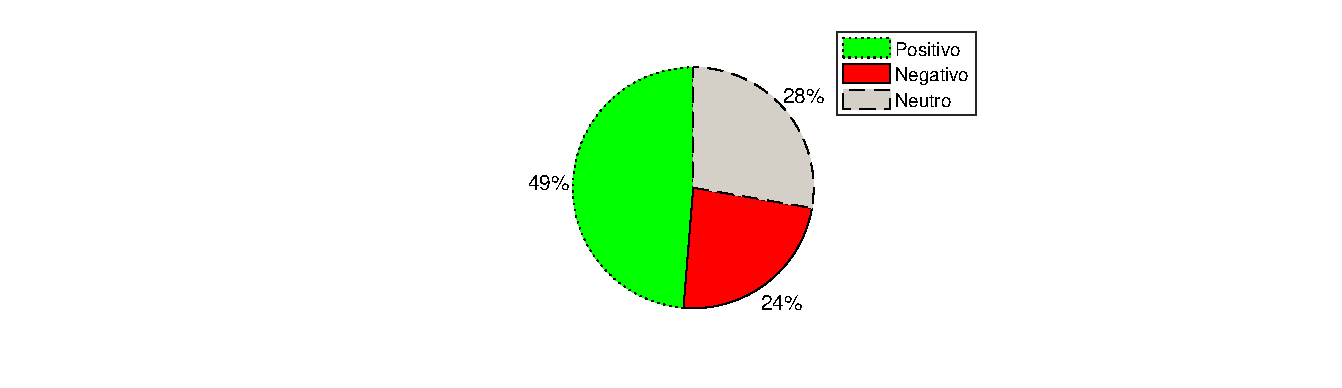
\epsfig{file=figuras/teste-4.eps, width=20cm}
	\caption{Quantidade de tweets separados por polaridade do teste 4. Fonte: Própria}
	\label{teste-graf-4}
\end{figure}
Segue abaixo um comparativo dos testes.

\begin{table}[]
	\caption{Comparando testes}
	\label{teste-comp}
	\resizebox{\textwidth}{!}{%
		\begin{tabular}{l|l|c|l|l|}
			\cline{2-5}
			\multicolumn{1}{c|}{} & \multicolumn{1}{c|}{Teste 1} & Teste 2 & \multicolumn{1}{c|}{Teste 3} & \multicolumn{1}{c|}{Teste 4} \\ \hline
			\multicolumn{1}{|l|}{Positivo} & 15517 & \multicolumn{1}{r|}{49263} & 47450 & 69070 \\ \hline
			\multicolumn{1}{|l|}{Negativo} & 17350 & 35079 & 7210 & 33461 \\ \hline
			\multicolumn{1}{|l|}{Neutro} & 108931 & \multicolumn{1}{l|}{57456} & 87138 & 39267 \\ \hline
			\multicolumn{1}{|l|}{Tempo (s)} & \multicolumn{1}{c|}{311.673} & 397.48 & 709.129 & 650.97 \\ \hline
		\end{tabular}%
	}
\end{table}

Com o comparativo analisado na tabela \ref{teste-comp} foi escolhido as configurações utilizadas no teste 4 para a realização da análise na base capturada.

\section{Resultados}\label{result}

Para a análise dos resultados é necessário o conhecimento de algumas premissas. O evento do Oscar 2016 foi a  88.ª cerimônia de entrega dos \textit{Academy Awards} em \textit{Los Angeles}, Estados Unidos. O evento teve duração de aproximadamente 4 horas com seu início na noite do dia 28 de fevereiro, as 20:00 horário de Brasília no tapete vermelho com a entrada dos artistas e convidados e  com seu encerramento as 2:00 do dia 29. OS marcos do evento são listados de acordo com a imagem \ref{time}

\begin{figure}[!h]
	\centering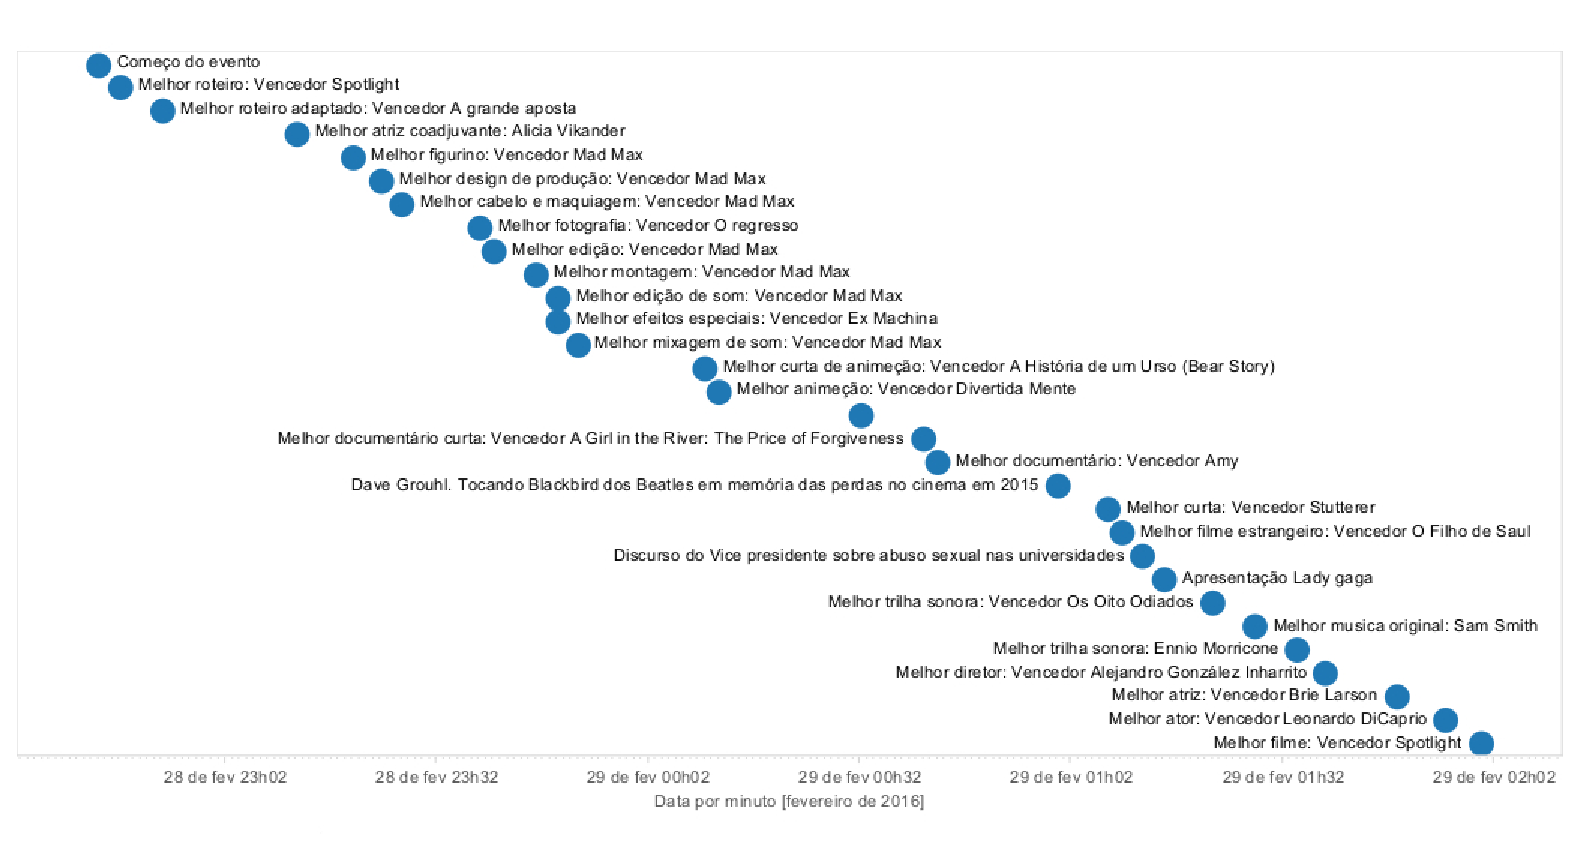
\epsfig{file=figuras/oscar_timeline.eps, width=15cm}
	\caption{Linha do tempo com os marcos do oscar 2016. Fonte:Folha de São Paulo}
	\label{time}
\end{figure}

\begin{figure}[!h]
	\centering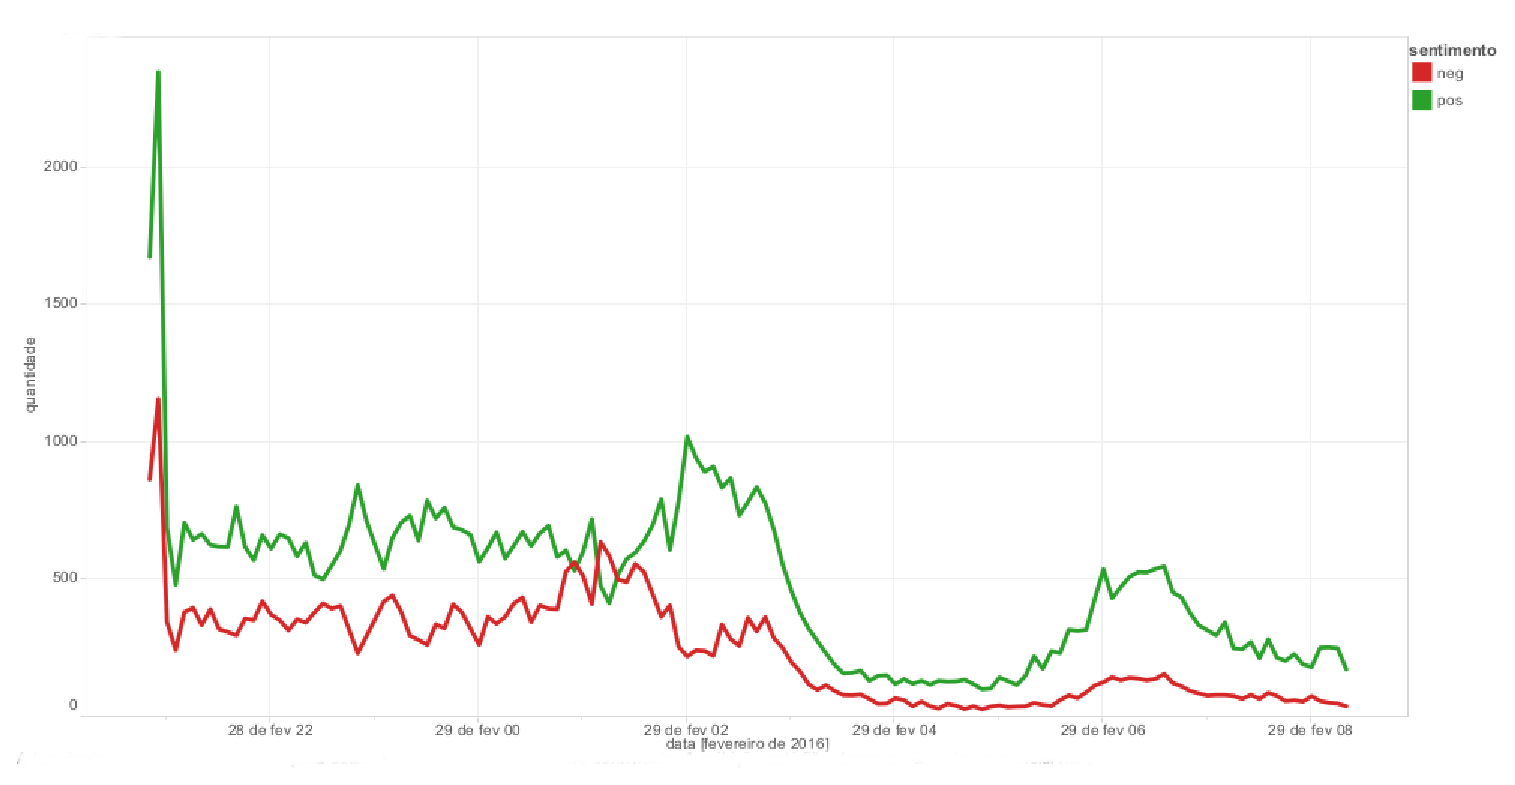
\epsfig{file=figuras/qtd_tweets_by_date.eps, width=15cm}
	\caption{Quantidade de tweets por tempo e polaridade. Fonte:Própria}
	\label{qtd}
\end{figure}
O grafico \ref{qtd} mostra como ficou a curva da quantidade de \textit{tweets} em relação ao tempo  dividido pela polaridade. Nele é visto um pico  no começo do evento, durante o tapete vermelho, nesse período foi visto que é onde ocorrem as maiores especulações sobre os ganhadores e indicados além das reações dos internautas com a entradas de seus artistas favoritos.

\begin{figure}[!h]
	\centering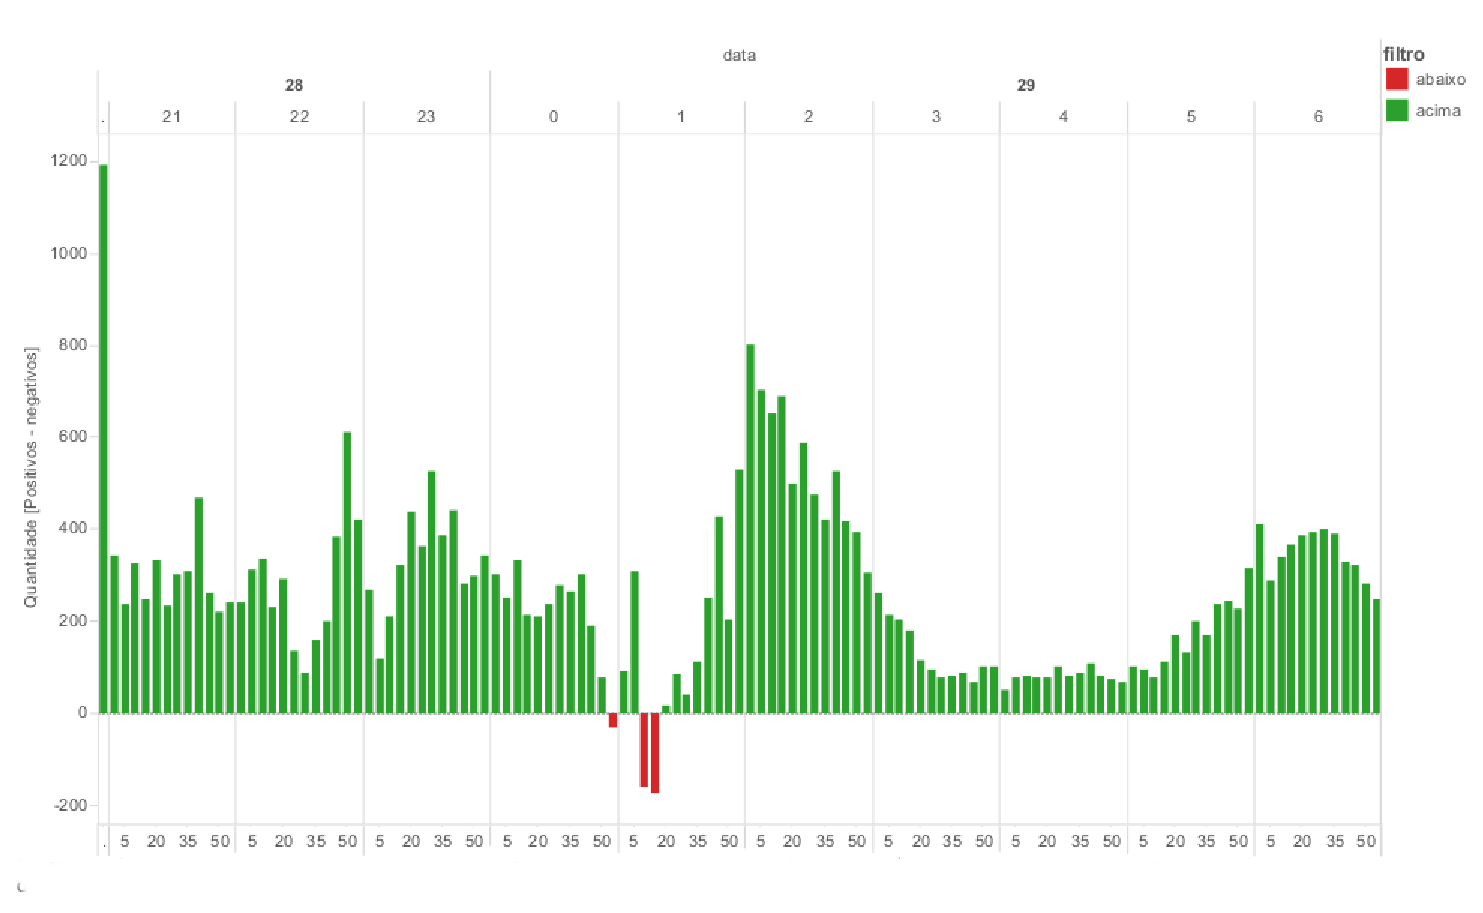
\epsfig{file=figuras/qtd_neg_pos.eps, width=15cm}
	\caption{Quantidade de tweets positivos diminuído pelos negativos pelo tempo. Fonte:Própria}
	\label{qtdnegpos}
\end{figure}

Analisando o gráfico \ref{qtd}, que possui uma visão mais macro, junto com o gráfico \ref{qtdnegpos}, com a visão mais micro, é notado que em dois momentos a quantidade de \textit{tweets} negativos sobrepõem a quantidade de positivos no primeiro momento é durante o \textit{show} do Dave Grohl onde é feita uma homenagem ao mortos no mundo do cinema em 2015 onde a sensação de luto ficou evidente durante a apresentação, e de acordo com \cite{freud1908conferencias}, é a reação à perda de objeto ou pessoa. Como afeto, o luto aproxima-se do humor depressivo. Com isso foi corraborado o aumento do sentimento negativo nessa parte do evento. Outro momento onde ocorre o mesmo efeito é Durante a apresentação da Lady Gaga onde o tema do filme onde música faz parte da trilha é sobre os estupros em faculdades americanas e mais uma vez esse aumento negativo é corraborado ao entender o tema pesado e sensível para as pessoas que sofreram e sofrem disso. Excluindo o pico no começo dos gráficos os maiores picos de positivos são presenciados as 2:00, vindo de uma crescente no final das 1:00 da manhã do dia 29 isso se deve a categorias mais aguardadas do evento que são:

 \begin{itemize}
 	\item Melhor atriz
 	\item Melhor ator
 	\item Melhor filme
 \end{itemize}

Sendo o que mais se destacou foi a premiação de melhor ator e a vitória de Leonardo DiCaprio que com seus 41 anos de idade e 26 de carreira nunca havia levado um prêmio de melhor ator da Academia. Essa vitória reflete nos gráficos de picos de positivos as 2:00 da manhã onde a repercusão da sua vitória é espelhada pelo twitter chegando aos \textit{trending topics} mundias na rede social.


\begin{figure}[!h]
	\centering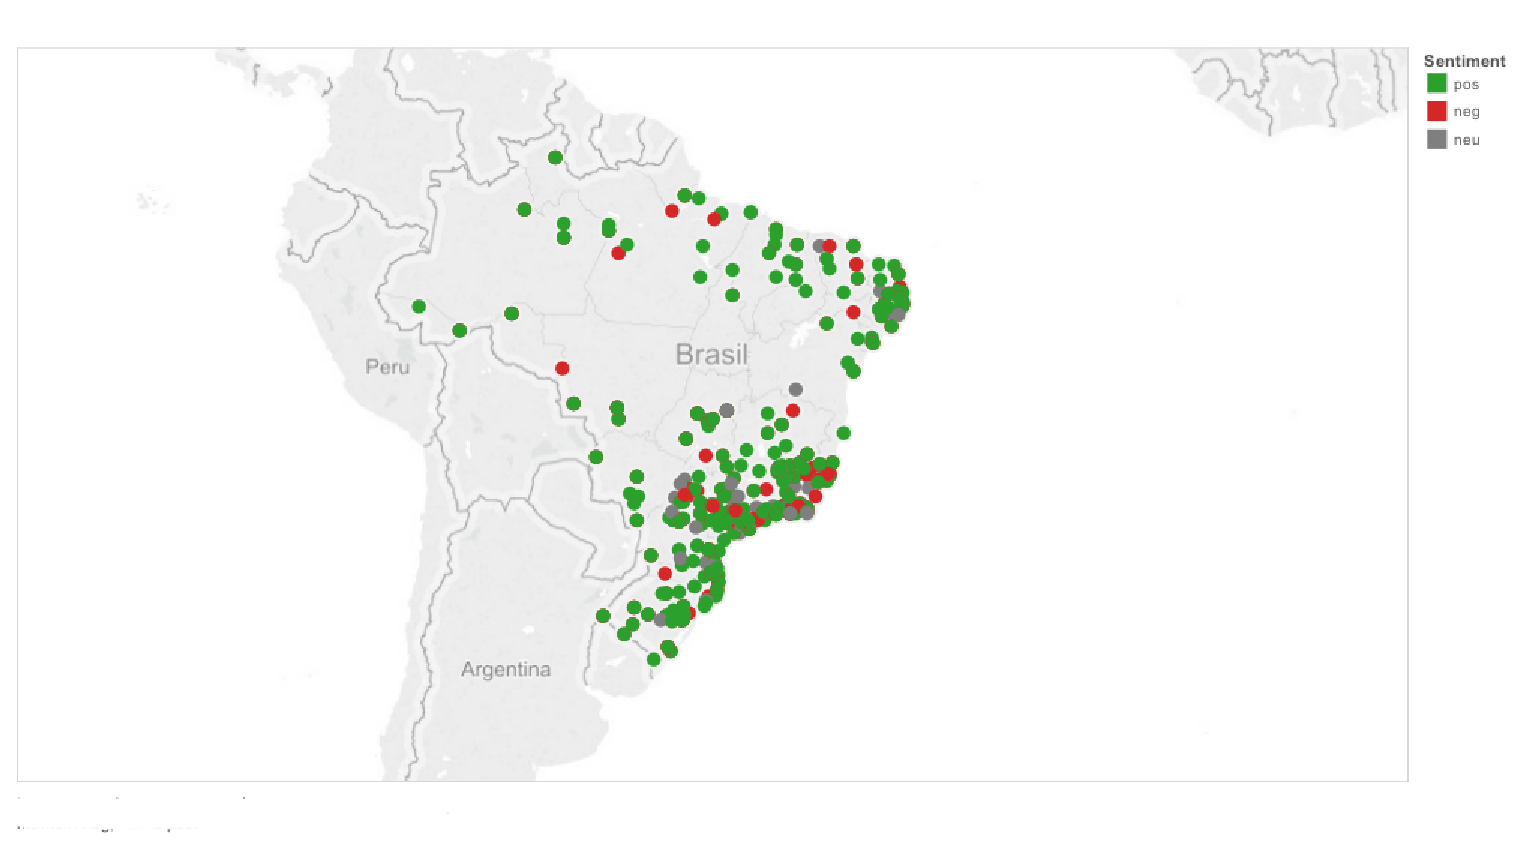
\epsfig{file=figuras/mapa.eps, width=15cm}
	\caption{Mapa de calor referente a polaridade de sentimento no Brasil. Fonte:Própria}
	\label{mapa}
\end{figure}
\chapter{Conclusão} \label{cap:conclusao}
%Um paragrágo relembrando a importancia do cenário
%Esse trabalho identificou e abordou alguns desses problemas, assim como propôs, desenvolveu e avaliou um serviço de gerenciamento eXXXXX
%Relembrar o que o trabalho fez.
%A proposta, XXX,  se destacou pelo XXXX que apresentou quando comparada XXXX. 
%A proposta atingiu os seguintes objetivos, exemplo:
%\begin{itemize}
%\item permitiu que sejam usados IEDs mais simples pois a solução não precisa ser implementada nesses dispositivos;
%\item reduziu o tempo de convergência dos algoritmos, o atraso na entrega de dados e o tráfego na rede;
%\item atendeu aos requisitos da Norma IEC 61850;
%\item implementou e testou um encaminhamento \textit{multicast} independente de camadas e transparente aos dispositivos finais;
%\item permitiu uma configuração da rede facilitada;
%\item usou o arquivo SCD da norma para autoconfiguração da rede de Telecomunicações;
%\item tornou a rede menos sujeita à erros por ser automático;
%\item permitiu o uso mais inteligente de recuperação de falhas;
%\item permitiu o alcance de tempos de resposta menores por possuir uma característica proativa.
%\end{itemize}
%Os experimentos e as análises realizadas mostraramXXXXXX
%Falar de todos os resultados encontrados de forma sumarzada, máximo de uma folha.
%Os testes mostraram, também, que 
%Outro ganho relacionado ao uso da técnica....
%A análise realizada mostra que ...

- Importância da mineração de opinião e oportunidades academicas e comerciais
- Desafio de implementação em língua portuguesa
- Solução aplicada para comprovar a viabilidade da mineração de opinião em língua portuguesa
- Relembrando:
-- Utilização do Twitter como plataforma de estudo
-- Criação de uma estrutura de coleta e armazenamento de messagens (tweets) sobre um determinado tema
-- Utilização de bases genéricas
-- Aplicação de técnicas de normalização de texto visando um maior desempenho ao classificar
-- Adaptação de um algoritmo de classificação conhecido (Naive Bayes)
-- Escolha do evento de premiação dos Oscars 2016 como estudo de caso inicial
-- Demonstração dos cenários de teste e seus impactos no resultado final
-- Análise do resultados obtidos através de gráficos 




\section{Trabalhos Futuros}\label{sec:8_trabfut}

Como visto neste trabalho, o algoritmo utilizado para gerar os resultados das classificações afim de realizar a análise de sentimento foi o \textit{Naive Bayes},. Para trabalhos futuros pode-se utilizar outros algoritmos como: Árvore de Decisão, Regressão Logística, \textit{Maximum Entropy Model}. Podendo ser usados somente o próprio algoritmo ou realizando um trabalho comparativo entre eles, descobrindo qual algoritmo gera melhores resultados.

Outro método que pode ser utilizado é a aplicação de \textit{n-grams}, para averiguar o melhor desempenho do modelo. Com isso poderia-se realizar testes de acurácia, que não foi o enfoque deste trabalho. Pode-se também utilizar outras fontes de dados, não só o Twitter, como: Facebook, fórums, comentários de sites ,entre outros. Mais um fator relevante são as bases, que nesse trabalho não tinham relação com o domínio estudado, pois eram genéricas, então pode-se realizar o mesmo trabalho com bases feitas específicas para o domínio.

Durante as pesquisas para esse trabalho foi encontrado um \textit{toolkit}  para a técnica de \textit{word embedding}, conhecido como \textit{word2vec}, criado em 2013 por uma equipe do Google. Esse tipo de técnica se baseia em redes neurais, que difere do algoritmo probabilístico utilizado nesse trabalho. Sendo essa uma outro proposta pra trabalhos futuros.

Por fim, pretende-se fazer o máximo para desenvolver o  processamento de linguagem natural para a língua portuguesa. Onde técnicas e métodos serão comparadas visando o melhor desempenho com uma análise mais profunda e a automação da inteligência artificial para o aproveitamento desse campo para o ser humano em suas tomadas de decisão. 



% --- -----------------------------------------------------------------
% --- Referencias Bibliograficas. (Obrigatorio)
% --- -----------------------------------------------------------------
\cleardoublepage
%\bibliographystyle{acm-2} 
%\bibliographystyle{abnt-num} % abbrv - abnt-num
\inputencoding{latin1}
\bibliographystyle{IEEEtran}
%\bibliographystyle{uff-ic}
\bibliography{referencia} % arquivo fonte com a bibliografia
%\bibliography{articles,books,standards,websites} % arquivo fonte com a bibliografia


%\addcontentsline{toc}{part}{Index}
%\printindex
\label{LastPage}
\end{document}